\section{Dark Side of Modalities: Reinforced Multimodal Distillation for Multimodal Knowledge Graph Reasoning (DSoM)}

\subsection{Bài toán và ý tưởng chính}

Đối với bài toán MKGR, ngoài cấu trúc quan hệ, mô hình còn có thể sử dụng những thông tin bổ sung như hình ảnh và văn bản để dự đoán thực thể còn thiếu. Tuy nhiên thì việc kết hợp nhiều phương thức không đồng nghĩa với việc toàn bộ các phương thức đều đóng góp tích cực cho mọi dự đoán. Ví dụ một phương thức có thể cung cấp thông tin hữu ích đối với thực thể này nhưng lại chứa thông tin nhiễu hoặc không liên quan tới thực thể khác.

Từ quan sát trên thì paper DSoM tiếp cận bài toán theo hướng chắt lọc tri thức (Knowledge Distillation - KD). (Knowledge Distillation còn có thể được dịch là chưng cất tri thức.) Tác giả xây dựng các mô hình teacher (giáo viên) sử dụng thông tin đa phương thức (cấu trúc, hình ảnh, văn bản) để dạy cho mô hình student (học sinh) mà mô hình student chỉ sử dụng thông tin về cấu trúc thay vì toàn bộ các phương thức khi suy luận. Mục tiêu tác giả muốn là giúp student học được những tín hiệu dự đoán hữu ích từ các teacher, không cần trực tiếp sử dụng phương thức bổ sung khác ngoài cấu trúc ở giai đoạn suy luận.

Ở paper này, tác giả không cố định một giáo viên hay kết hợp các giáo viên theo cùng một cách cho toàn bộ dữ liệu (vì như lập luận đầu tiên phía trên, mô hình có thể tiếp nhận cả những dự đoán thiếu chính xác cho một số điểm dữ liệu nào đó). Vì vậy tác giả sử dụng học tăng cường (Reinforcement Learning - RL) để lựa chọn và kết hợp các giáo viên theo từng truy vấn. Cơ chế này giúp student học từ những nguồn tri thức phù hợp hơn với từng trường hợp cụ thể và không xem mọi phương thức đều có giá trị như nhau.




Ngoài việc lựa chọn giáo viên, DSoM còn phân biệt tri thức liên quan đến các thực thể là đáp án đúng đã biết (neighbors) và các thực thể chưa được ghi nhận là đáp án đúng (non-neighbors).

Tác giả đề xuất Neighbor-Decoupled Knowledge Distillation (NDKD) nhằm phân tách quá trình truyền tri thức từ teacher sang student theo hai nhóm thực thể này.

Lưu ý: non-neighbors không nhất thiết là đáp án sai. Do đồ thị tri thức có thể chưa
hoàn chỉnh, một thực thể không thuộc tập neighbors chỉ có nghĩa là quan hệ tương ứng chưa được ghi nhận trong dữ liệu đang xét.

Hai thành phần này tạo nên ý tưởng chính của DSoM: lựa chọn nguồn tri thức phù hợp và chuyển giao tri thức đó cho mô hình chỉ
sử dụng cấu trúc.

Như minh họa ở Hình~\ref{fig:dsom_motivation},
việc kết hợp nhiều phương thức không phải lúc nào
cũng cải thiện chất lượng dự đoán.

\begin{figure}[t]
    \centering
    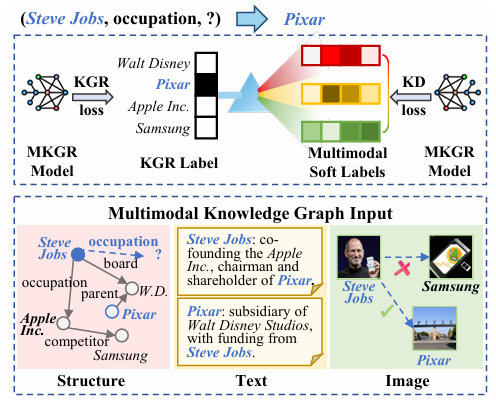
\includegraphics[width=\linewidth]{figures/fig1_dsom.png}
    \caption{Minh họa những hạn chế khi kết hợp các phương thức
    trong suy luận trên đồ thị tri thức đa phương thức và vai trò
    của tri thức từ phân phối dự đoán.  Nguồn: \cite{10.1145/3746027.3754576}, Hình 1.}
    \label{fig:dsom_motivation}
\end{figure}

Về tên của paper, nhóm hiểu tác giả đặt tên ``Dark Side of Modalities'' có nghĩa là sự ảnh hưởng tiêu cực khi một số phương thức có thể chứa thông tin nhiễu, không liên quan như phân tích ở đoạn đầu tiên. Và tác giả cũng định nghĩa ``Dark Knowlegde'' là tri thức ẩn trong phân phối dự đoán. Student không chỉ học đáp án đúng mà học cả phân phối logit từ teacher.

Nhóm phân tích cơ chế lựa chọn tổ hợp giáo viên RC theo bốn thành phần của học tăng cường: trạng thái, hành động, phần thưởng và chính sách.

\subsection{Phương pháp DSoM}

Kiến trúc tổng thể của DSoM được trình bày trong
Hình~\ref{fig:dsom_framework}. Phương pháp gồm
ba thành phần chính: xây dựng các mô hình giáo viên
theo từng phương thức, lựa chọn tổ hợp giáo viên
bằng học tăng cường và truyền tri thức sang mô hình
học sinh thông qua NDKD.

\begin{figure*}[t]
    \centering
    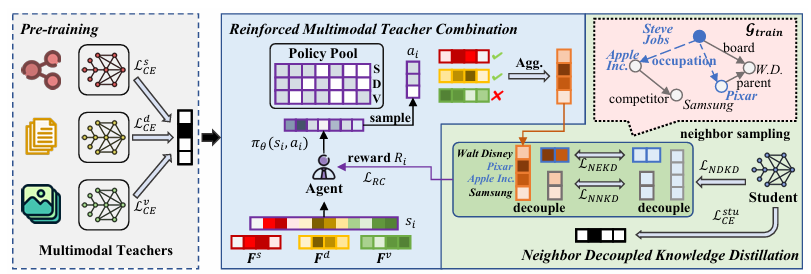
\includegraphics[width=\textwidth]{figures/fig2_dsom.png}
    \caption{Kiến trúc tổng thể DSoM gồm ba giai đoạn:
    huấn luyện các mô hình giáo viên theo từng phương thức,
    lựa chọn tổ hợp giáo viên bằng Reinforced Combination (RC)
    và truyền tri thức sang mô hình học sinh bằng
    Neighbor-Decoupled Knowledge Distillation (NDKD).
     Nguồn: \cite{10.1145/3746027.3754576}, Hình 2.}
    \label{fig:dsom_framework}
\end{figure*}


\subsubsection{Xây dựng các mô hình giáo viên và học sinh}

Để thực hiện Knowlegde Distillation, tác giả sẽ xây dựng các mô hình teacher và student. Trong paper, tác giả xây dựng ba teacher, mỗi teacher sẽ được học từ một nguồn phương thức tương ứng. Cụ thể là một teacher học từ thông tin cấu trúc (structure),
một teacher học thông tin từ hình ảnh (visual), và một teacher cuối học từ văn bản (textual). Các teacher được huấn luyện trước để dự đoán thực thể còn thiếu.  Theo cách hiểu của nhóm, việc phân chia như vậy giúp mô hình giữ lại được những góc nhìn khác nhau khi đánh giá cùng một truy vấn, thay vì kết hợp toàn bộ
thông tin ngay từ đầu.

Đối với các thông tin về hình ảnh và văn bản, tác giả sử dụng model pretrained như ViT và BERT để trích xuất đặc trưng. Các model này không trainable trong pipeline của DSoM mà chỉ tạo ra các vector đặc trưng ban đầu. Sau đó các vector đặc trưng này mới được đưa qua các lớp phép chiếu (projection layer) để model dự đoán thực thể còn thiếu. Các projection layer này có những tham số có thể học (trainable weights) trong quá trình huấn luyện teacher.

Xét một truy vấn $(h,r,?)$, mỗi teacher đều đưa
ra điểm dự đoán cho tất cả thực thể ứng viên trong tập
$E$. Ta ký hiệu kết quả của teacher thuộc phương thức
$m$ là:

\begin{equation}
F_m(h,r)=[f_m(h,r,e)]_{e\in E}.
\end{equation}

$f_m(h,r,e)$ là điểm của teacher $m$ đánh giá
mức độ phù hợp của thực thể $e$ với truy vấn $(h,r,?)$.
Kết quả mà teacher cho được không phải là
một thực thể được dự đoán, mà là một vector logits
chứa điểm của toàn bộ các thực thể ứng viên.

Các teacher sử dụng ComplEx để tính điểm dự đoán và
được huấn luyện với hàm loss là cross-entropy. Sau khi hoàn thành
huấn luyện, các logits của teacher được sử dụng để
hướng dẫn student.

Đối với student, tác giả sử dụng một mô hình chỉ học
embedding của thực thể và quan hệ từ cấu trúc
với hàm chấm điểm ComplEx tương tự như teacher. Điểm
khác biệt là student không trực tiếp sử dụng đặc trưng
hình ảnh hay văn bản.

Tác giả nói rằng việc lựa chọn mô hình student như vậy không đồng nghĩa với việc loại bỏ hoàn toàn thông tin đa phương thức, mà tác giả muốn truyền gián tiếp thông tin này qua quá trình distillation. Theo nhóm thì cách thiết kế này có lợi ích giảm sự phụ thuộc vào dữ liệu đa phương thức ở giai đoạn inference. Trong thực tế thì không phải thực thể nào cũng có đủ hình ảnh và văn bản mô tả đi kèm. 


\subsubsection{Lựa chọn tổ hợp giáo viên bằng học tăng cường}

Sau khi huấn luyện ba teacher, tác giả đề xuất
cơ chế Reinforced Combination (RC), sử dụng
học tăng cường (Reinforcement Learning - RL)
để lựa chọn và kết hợp các teacher phù hợp
với từng truy vấn.

Trong cơ chế này, agent không trực tiếp thực hiện bài toán MKGR, tức không dự đoán thực thể còn thiếu. Thay vào đó, agent quyết định những teacher nào sẽ tham gia hướng dẫn student thông qua quá trình Knowledge Distillation.


Để hiểu cách học tăng cường được áp dụng để chọn teacher hợp lý, nhóm phân tích bài toán qua các thành phần state,action, reward và policy.

\textit{a) Trạng thái (State):}


Agent cần có thông tin để quyết định nên lựa chọn teacher nào. Trạng thái trong DSoM được tạo bằng cach nối 3 vector logits của ba teacher:

\begin{equation}
s_i=[F_s\|F_v\|F_d].
\end{equation}

$F_s$, $F_v$ và $F_d$ lần lượt là logits
của teacher cấu trúc, hình ảnh và văn bản; ký hiệu
$\|$ biểu diễn phép nối vector.

Agent không trực tiếp nhận hình ảnh hay văn bản gốc. Thay vào đó, agent quan sát
kết quả dự đoán mà các teacher đưa ra. 

Nhóm thấy rằng cách thiết kế này hợp lý với mục tiêu
lựa chọn teacher. Vì thông tin cuối cùng được truyền
cho student chính là logits, nên agent sử dụng
logits để đánh giá sự khác biệt giữa các teacher
thay vì phải xử lý lại dữ liệu của từng phương thức.

\textit{b) Hành động (Action):}

Sau khi nhận trạng thái, agent phải quyết định sẽ
sử dụng những teacher nào.

Với ba teacher, mỗi teacher có hai khả năng là được
chọn hoặc không được chọn. Như vậy sẽ có $2^3=8$
tổ hợp, trừ đi một trường hợp không teacher nào được chọn, nên số hành động thực tế trong không gian
hành động của agent là:


\begin{equation}
|\mathcal{A}|=2^3-1=7.
\end{equation}

Ví dụ: Agent có thể lựa chọn riêng teacher
cấu trúc, kết hợp cấu trúc với văn bản, hoặc sử
dụng cả ba teacher,...

Tác giả sử dụng một mạng MLP để học phân phối xác
suất lựa chọn các tổ hợp này. Với trạng thái $s_i$,
agent lấy mẫu một hành động theo policy:

\begin{equation}
a_i\sim\pi_\theta(a\mid s_i).
\end{equation}




Sau khi xác định những teacher được chọn, tác giả lấy trung bình logits của chúng:

\begin{equation}
F_{\mathrm{tea}}^{(i)}
=
\frac{1}{|\mathcal{M}_i|}
\sum_{m\in\mathcal{M}_i}F_m^{(i)}.
\ 
\end{equation}

Trong đó, \(\mathcal{M}_i\) là tập teacher được agent lựa chọn cho mẫu huấn luyện thứ \(i\). Qua đối chiếu mã nguồn, agent thực hiện lựa chọn tổ hợp teacher riêng cho từng mẫu dữ liệu chứ không sử dụng một tổ hợp cố định cho toàn bộ batch. Nhiệm vụ của agent là học cách lựa chọn tổ hợp phù hợp, thay vì trực tiếp học trọng số kết hợp của từng teacher.

Sự khác biệt của phương pháp này so với cách kết hợp bằng trọng số là agent lựa chọn một trong bảy tổ hợp teacher có trước; và các teacher được chọn có trọng số bằng nhau. Chẳng hạn, nếu chọn Structure và Visual, DSoM sẽ lấy trung bình logits của hai teacher với trọng số là 0.5 và 0.5. Còn phương pháp kết hợp trọng số có thể học được giá trị như 0.75 và 0.25, nghĩa là structure đóng góp nhiều hơn visual. (Đã xác nhận điều này trong source code.)

\textit{c) Phần thưởng (Reward):}


Để biết một tổ hợp teacher được lựa chọn tốt hay không, nhóm sẽ trình bày
qua phần reward. Reward chính là tín hiệu dùng để đánh giá hành động của agent. Trong paper, tác giả sử dụng
Cross-Entropy để so sánh kết quả dự đoán của tổ hợp teacher với student:


\begin{equation}
R_i=
\begin{cases}
+1, & CE_{\mathrm{tea}}<CE_{\mathrm{stu}},\\
-10, & \text{ngược lại}.
\end{cases}
\end{equation}

$CE_{\mathrm{tea}}$ và $CE_{\mathrm{stu}}$
là Cross-Entropy của dự đoán từ tổ hợp teacher và
student đối với nhãn của mẫu đang xét.

Nếu tổ hợp teacher có Cross-Entropy thấp hơn student, agent được thưởng $+1$, ngược lại bị phạt $-10$. Vì student liên tục được cập nhật, cùng một tổ hợp teacher có thể nhận reward khác nhau trong quá trình huấn luyện.

Nhóm nhận thấy mức phạt lớn gấp mười lần mức thưởng, cho thấy tác giả muốn hạn chế việc lựa chọn những teacher dự đoán kém hơn student. Tuy nhiên, paper chưa giải thích rõ lý do lựa chọn hai giá trị $+1$ và $-10$ này.

Reward được tác giả tính bằng Cross-Entropy, chứ không trực tiếp sử dụng các
metric đánh giá MKGR như MRR hoặc Hits@K. Do đó,
agent đang học cách lựa chọn teacher dựa trên chất
lượng dự đoán theo Cross-Entropy, còn việc lựa chọn
này có cải thiện thứ hạng thực thể hay không cần
được đánh giá thực nghiệm.

\textit{d) Cập nhật chính sách (Policy):}


Sau khi nhận reward, agent sẽ cập nhật policy để những hành động có lợi có khả năng được chọn cao hơn trong các lần tiếp theo. Tác giả sử dụng Policy Gradient để cập nhật policy này. Ngoài reward của tổ hợp được chọn, mô hình còn xây dựng baseline bằng cách lấy trung bình logits của ba teacher rồi tính reward tương ứng.


Sự chênh lệch giữa reward của hành động và reward
baseline được ký hiệu:

\begin{equation}
\delta_i=R_i-\hat{R}_i.
\end{equation}

Ký hiệu $\hat{R}_i$ là phần thưởng baseline.
Giá trị $\delta_i$ được sử dụng khi cập nhật policy
để giảm phương sai của ước lượng gradient.

Hàm mất mát huấn luyện agent được viết:

\begin{equation}
\mathcal{L}_{RC}
=-\frac{1}{|\mathcal{T}_{train}|}
\sum_i \delta_i\log\pi_\theta(a_i\mid s_i).
\end{equation}

Nếu $\delta_i$ dương, việc tối thiểu hóa hàm mất
mát sẽ khuyến khích tăng xác suất của hành động
đã chọn. Ngược lại, khi $\delta_i$ âm, xác suất
của hành động đó sẽ bị giảm.

Toàn bộ quá trình RL trong DSoM có thể
được hiểu như sau: agent nhận các logits của ba
teacher, lựa chọn một tổ hợp, sử dụng kết quả tổ
hợp để tính reward, sau đó cập nhật policy. Agent không học cách trả
lời trực tiếp truy vấn $(h,r,?)$, mà học cách
lựa chọn nguồn tri thức để hỗ trợ student.

\subsubsection{Neighbor-Decoupled Knowledge Distillation}


Agent đã lựa chọn teacher và tạo ra logits tổng hợp, bước tiếp theo là chuyển những thông tin này sang student. Nếu chỉ lấy thực thể có điểm dự đoán cao nhất từ teacher làm nhãn huấn luyện, student sẽ không học được toàn bộ thông tin trong phân phối dự đoán. Tác giả sử dụng Knowledge Distillation cũng chính vì muốn student học được thông tin trong phân phối dự đoán này.


Logits của teacher và student được
chuyển thành phân phối xác suất thông qua softmax
với tham số nhiệt độ (temperature) $\tau$:

\begin{equation}
\begin{aligned}
P_{\mathrm{tea}}&=
\operatorname{softmax}(F_{\mathrm{tea}}/\tau),\\
P_{\mathrm{stu}}&=
\operatorname{softmax}(F_{\mathrm{stu}}/\tau).
\end{aligned}
\end{equation}








Trong MKGR, một truy vấn có thể có nhiều đáp án đúng. Ví dụ với truy vấn $(A,r,?)$, nếu đồ thị tồn tại hai bộ ba $(A,r,B)$ và $(A,r,C)$ thì cả $B$ và $C$ đều là đáp án đúng. Nếu chỉ xét bộ ba $(A,r,B)$, thực thể $C$ có thể bị xem là một đáp án không đúng, mặc dù nó cũng có quan hệ $r$ với $A$.

Trong Knowledge Distillation, phương pháp Decoupled Knowledge Distillation (DKD) phân tách việc học thành thông tin của nhãn đích và các nhãn còn lại. Tuy nhiên, cách phân tách này chưa phù hợp với đặc điểm nhiều đáp án đúng của MKGR. Vì vậy, tác giả đề xuất Neighbor-Decoupled Knowledge Distillation (NDKD), trong đó thay vì chỉ xét một đáp án đúng, mô hình xét toàn bộ tập neighbors:

\[
\mathcal{N}(h,r)=
\{e\mid(h,r,e)\in\mathcal{T}_{train}\}.
\]

Đây là tập các thực thể có quan hệ $r$ với $h$ trong tập huấn luyện. Những thực thể không thuộc tập này được gọi là non-neighbors.

Nhóm lưu ý rằng non-neighbors không nhất thiết
là những đáp án sai trong thế giới thực. Do KG
có thể chưa hoàn chỉnh, một thực thể không có
trong tập neighbors chỉ có nghĩa quan hệ tương
ứng chưa được ghi nhận trong dữ liệu đang xét.

Sau khi chia các thực thể thành hai nhóm, tác
giả xây dựng hai thành phần loss.










\textit{a) Neighbor Entity Knowledge Distillation (NEKD):}

Thành phần NEKD giúp student học cách teacher đánh giá nhóm neighbors, thay vì chỉ tập trung vào một đáp án đúng.

Chẳng hạn, với truy vấn $(A,r,?)$, giả sử $B$ và $C$ là hai neighbors. Teacher dự đoán xác suất của $B$ và $C$ lần lượt là $0.4$ và $0.3$, trong khi student dự đoán $0.2$ và $0.1$.

Theo công thức trong paper, tác giả lấy trung bình xác suất của các neighbors:

\begin{equation}
p_{\mathcal{N}}=
\frac{1}{|\mathcal{N}|}
\sum_{e\in\mathcal{N}}p_e.
\label{eq:nekd_mean}
\end{equation}

Với ví dụ trên, teacher có xác suất trung bình là $0.35$, còn student là $0.15$. Từ đó, tác giả tạo hai phân phối nhị phân:

\begin{equation}
\begin{aligned}
b_{\mathrm{tea}}&=[0.35,0.65],\\
b_{\mathrm{stu}}&=[0.15,0.85].
\end{aligned}
\end{equation}

Hai phân phối này được so sánh bằng KL Divergence:

\begin{equation}
\mathcal{L}_{NEKD}
=KL(b_{\mathrm{tea}}\|b_{\mathrm{stu}}).
\end{equation}

NEKD giúp student điều chỉnh xác suất dành cho nhóm neighbors sao cho gần với teacher hơn.

Công thức~\eqref{eq:nekd_mean} và ví dụ trên trình bày
cách lấy trung bình xác suất của các thực thể thuộc nhóm
neighbors theo bài báo gốc. Tuy nhiên, theo tài liệu giao thức
thực nghiệm của repository, mã nguồn được sử dụng trong
các lần tái lập tính xác suất nhóm neighbors bằng phép tổng:

\begin{equation}
    p_N^{\mathrm{impl}} = \sum_{e \in N} p_e,
    \label{eq:nekd_sum}
\end{equation}

\noindent
sau đó xây dựng phân phối nhị phân
$\left[p_N^{\mathrm{impl}},\,1-p_N^{\mathrm{impl}}\right]$.
Hai cách tính khác nhau khi tập neighbors có nhiều hơn
một phần tử. Do đó, cần phân biệt công thức trình bày
theo bài báo với cách triển khai thực tế được sử dụng
để tạo ra các kết quả tái lập.

Một vấn đề mà nhóm nhận ra ở đây là phân phối xác suất của các neighbors được đại diện bởi một giá trị trung bình, nên có thể làm mất thông tin về xác suất của từng thực thể. Ví dụ 1 tập neighbor là $\{A,B,C\}$ có 3 phần tử, teacher dự đoán $[0.3,0.2,0.1]$ và student dự đoán $[0.1,0.3,0.2]$ vẫn cho NEKD loss bằng $0$ (vì trung bình cả hai đều là $0.2$), mặc dù xác suất của từng neighbor khác nhau. Tuy nhiên, điều này chưa hẳn là hạn chế, vì các neighbors đều là đáp án đúng và không nhất thiết phải có cùng thứ tự ưu tiên.

\textit{b) Non-Neighbor Knowledge Distillation
(NNKD):}

Thành phần thứ hai tập trung vào các thực thể không thuộc tập neighbors.

Tác giả chuẩn hóa lại xác suất của những thực thể non-neighbors để tạo thành một phân phối riêng:

\begin{equation}
\tilde{p}_e=
\frac{p_e}
{\sum_{j\notin\mathcal{N}}p_j},
\quad e\notin\mathcal{N}.
\end{equation}

Sau đó student được hướng dẫn học phân phối này từ teacher thông qua:

\begin{equation}
\mathcal{L}_{NNKD}
=KL(\widetilde{P}_{\mathrm{tea}}
\|\widetilde{P}_{\mathrm{stu}}).
\end{equation}

Đây là thành phần thể hiện khá rõ
ý tưởng Dark Knowledge của tác giả.

Ví dụ, trong tập non-neighbors có ba thực thể
$\{D,E,F\}$. Mặc dù cả ba đều không thuộc
tập đáp án đúng đã biết, teacher có thể đánh
giá $D$ phù hợp với truy vấn hơn $E$, và $E$
phù hợp hơn $F$.

Nếu chỉ học nhãn đúng hoặc sai, student không
nhận được đầy đủ những thông tin này. Nhưng
khi học phân phối của teacher, student có thể
học thêm mức độ phù hợp tương đối giữa các
thực thể không phải đáp án đích.

NNKD không cần khẳng định các non-neighbors đều thực sự
sai. Thành phần này khai thác sự khác biệt
trong cách teacher đánh giá những thực thể
chưa được ghi nhận là đáp án đúng.

Cuối cùng, hai thành phần được kết hợp:

\begin{equation}
\mathcal{L}_{NDKD}
=\alpha\mathcal{L}_{NEKD}
+\beta\mathcal{L}_{NNKD}.
\end{equation}

$\alpha$ và $\beta$ là các hệ số điều chỉnh đóng góp của từng thành phần.

Đóng góp chính của NDKD không phải là việc sử dụng KL Divergence (kỹ
thuật này đã phổ biến trong Knowledge Distillation) mà là điều chỉnh
cách phân tách phân phối xác suất để phù hợp
với trường hợp một truy vấn có nhiều đáp án
đúng trong MKGR.

Nhóm cho rằng hiệu quả của
cách phân tách này phụ thuộc vào chất lượng
của tập neighbors được ghi nhận. Nếu dữ liệu
huấn luyện còn thiếu nhiều quan hệ, một số
đáp án thực sự đúng vẫn có thể bị đưa vào
tập non-neighbors.

\subsubsection{Hàm mất mát và quy trình huấn luyện}

Sau khi phân tích hai thành phần trên, nhóm
tổng hợp lại quy trình huấn luyện của DSoM.

Đầu tiên, ba teacher được huấn luyện trước,
mỗi teacher khai thác một phương thức khác
nhau. Sau đó, student được khởi tạo để học
từ nhãn thực tế của bài toán MKGR và từ
phân phối dự đoán của các teacher.

Trong quá trình huấn luyện student, agent
nhận logits từ ba teacher để lựa chọn tổ
hợp phù hợp. Các logits được chọn được lấy
trung bình số lượng teacher trong tổ hợp, sau đó sử dụng trong NDKD để
hướng dẫn student.

Đồng thời, agent nhận reward từ việc so
sánh Cross-Entropy giữa tổ hợp teacher
và student để cập nhật policy của mình.

Hàm mục tiêu tổng thể trong paper là:

\begin{equation}
\mathcal{L}_{stu}
=\mathcal{L}^{stu}_{CE}
+\mathcal{L}_{RC}
+\gamma\mathcal{L}_{NDKD}.
\end{equation}

Trong đó, $\mathcal{L}^{stu}_{CE}$ là loss
dự đoán thực thể của student,
$\mathcal{L}_{RC}$ là loss của agent và
$\mathcal{L}_{NDKD}$ là loss dùng để truyền
tri thức từ teacher sang student. Hệ số
$\gamma$ điều chỉnh mức đóng góp của NDKD.

Dù được viết chung trong hàm mục tiêu, các thành phần
này đảm nhận những nhiệm vụ khác nhau.
Loss của agent dùng để học chính sách lựa
chọn teacher, còn Cross-Entropy và NDKD
được sử dụng để huấn luyện student.

Cuối cùng, ở giai đoạn inference, tác giả
chỉ sử dụng student. Các teacher và agent
không còn tham gia vào việc dự đoán thực
thể còn thiếu.

Như vậy, theo cách hiểu của nhóm, DSoM
có thể được nhìn nhận qua hai câu hỏi:
student nên học từ những teacher nào,
và student nên học những thông tin gì
từ kết quả dự đoán của các teacher đó?

Reinforced Teacher Combination giải quyết
câu hỏi thứ nhất thông qua học tăng cường,
còn NDKD giải quyết câu hỏi thứ hai thông
qua việc phân tách phân phối dự đoán.

Đây cũng là hai thành phần mà nhóm cho
rằng thể hiện rõ nhất ý tưởng của tác giả
trong công trình DSoM.

\subsection{Tái lập thực nghiệm}

\subsubsection{Thiết lập thực nghiệm}

Nhóm sử dụng mã nguồn công khai của DSoM và bổ sung các script chuẩn bị dữ liệu (vì code do tác giả công bố bị thiếu nhiều thành phần liên quan đến chuẩn bị dataset, các hàm phụ trợ,...). Nhóm đánh giá và theo dõi kết quả bằng W\&B.
Mã nguồn tái lập được công bố tại
\href{https://github.com/keiranoluv/Reproduce_DSoM}{GitHub}.

Thực nghiệm được thực hiện trên GPU NVIDIA
GeForce RTX 5090, Python 3.12,
PyTorch 2.7.0 (CUDA 12.8), với random seed 2022.
Cấu hình chính gồm rank 2000, batch size 1000,
optimizer Adagrad với learning rate 0.1,
regularization N3 bằng 0.01, tối đa 200 epochs,
validation mỗi 3 epochs và early stopping
patience 10. Student sử dụng KD temperature 4,
trọng số KD bằng 2 và $\alpha=\beta=1$.

Nhóm tái lập trên sáu bộ dữ liệu gồm DB15K,
MKG-W, MKG-Y, FB15K-237, WN18 và WN9.
Teacher sử dụng thông tin cấu trúc, hình ảnh
và văn bản, trong khi student chỉ sử dụng
thông tin cấu trúc. Các đặc trưng hình ảnh
và văn bản được tái tạo bằng ViT và BERT.

Nhóm bổ sung pipeline trích xuất đặc trưng ảnh do mã nguồn công
khai chưa cung cấp script tương ứng. Tuy nhiên, pipeline tái lập
sử dụng đầu vào $384\times384$, khác với cấu hình
\texttt{vit-base-patch16-224} được tác giả công bố.
Đây là sai khác trong triển khai của nhóm; ảnh hưởng đến kết quả
chưa được định lượng.

Checkpoint của teacher được chọn theo
validation Hits@10, còn checkpoint của
student được chọn theo validation MRR.
Các kết quả test được lấy từ
\texttt{final\_result} của checkpoint
được chọn thay vì metric ở epoch cuối.

Giới hạn về dữ liệu: Tập validation của DB15K trong nguồn dữ liệu công khai có các bộ ba trùng với tập huấn luyện và tập kiểm tra. Nhóm giữ nguyên cách chia dữ liệu này trong các thực nghiệm đối chiếu. Do validation được sử dụng để chọn checkpoint, sự trùng lặp làm giảm tính độc lập của quá trình lựa chọn mô hình và có thể khiến kết quả đánh giá lạc quan hơn. Vì vậy, các kết quả trên DB15K cần được diễn giải cùng giới hạn này.

Nhóm sử dụng ba chế độ thực nghiệm:

\begin{itemize}
    % \item \texttt{source\_frozen}: Giữ nguyên mã nguồn công khai tác giả công bố. Vấn đề trong mã nguồn này là agent có lựa chọn tổ hợp teacher nhưng policy không được cập nhật do thiếu tham số trong optimizer - đây là điểm không khớp giữa paper và mã nguồn.
    \item \texttt{source\_frozen}: giữ cách cập nhật tham số của mã nguồn
        công khai DSoM tại commit \texttt{171e59c}. Policy vẫn nhận
        logits của teacher và lấy mẫu tổ hợp bằng
        \texttt{torch.multinomial}.
        \footnote{\href{https://github.com/OreOZhao/DSoM/blob/171e59cb069d50abf039fa824b079e23b8956696/src/kd.py\#L337-L354}{DSoM: tính phân phối policy và lấy mẫu tổ hợp.}}
        Tuy nhiên, \texttt{get\_learnable\_parameters} chỉ trả về tham
        số student, còn optimizer được khởi tạo từ danh sách này,
        nên tham số mạng policy không được cập nhật.
        \footnote{\href{https://github.com/OreOZhao/DSoM/blob/171e59cb069d50abf039fa824b079e23b8956696/src/kd.py\#L22-L24}{DSoM: danh sách tham số được tối ưu};
        \href{https://github.com/OreOZhao/DSoM/blob/171e59cb069d50abf039fa824b079e23b8956696/src/kd_learn.py\#L246-L255}{khởi tạo optimizer}.}
        Do đó, ``frozen'' chỉ việc giữ nguyên tham số policy, không
        đồng nghĩa luôn chọn một tổ hợp teacher cố định. Các kết quả
        này chưa chứng minh hiệu quả của việc học policy bằng RL.
    \item \texttt{learned\_RC}: Bổ sung optimizer riêng để huấn luyện policy theo cơ chế RL giống mô tả của paper;
    \item \texttt{fixed\_teacher}: Sử dụng một teacher hoặc tổ hợp cố định, không qua agent. Sự phân biệt này giúp đánh giá riêng khả năng tái lập mã nguồn và hiệu quả của cơ chế RL được đề xuất trong paper.
\end{itemize}

Để đánh giá khả năng tái lập và kiểm chứng
các thành phần của DSoM, nhóm tổ chức
thực nghiệm theo Bảng~\ref{tab:dsom_exp_overview}.

\begin{table}[htbp]
\centering
\caption{Tổng quan các nhóm thực nghiệm DSoM.}
\label{tab:dsom_exp_overview}
\scriptsize
\setlength{\tabcolsep}{3pt}
\renewcommand{\arraystretch}{1.2}

\begin{tabular}{@{}
>{\raggedright\arraybackslash}p{0.27\columnwidth}
>{\raggedright\arraybackslash}p{0.45\columnwidth}
>{\raggedright\arraybackslash}p{0.20\columnwidth}@{}}

\toprule
\textbf{Thực nghiệm}
& \textbf{Mục tiêu}
& \textbf{Bảng đối chiếu so với paper} \\
\midrule

Benchmark
& Đối chiếu chất lượng dự đoán trên
sáu bộ dữ liệu.
& Tables 1, 3, 7 \\

\addlinespace
Teacher selection
& So sánh các chiến lược
lựa chọn teacher.
& Table 2 \\

\addlinespace
Component ablation
& Đánh giá vai trò của RC,
NEKD và NNKD.
& Table 4 \\

\addlinespace
Modality ablation
& Đánh giá đóng góp của từng
nguồn thông tin.
& Table 6 \\


\bottomrule
\end{tabular}
\end{table}




Nhóm còn thực hiện các thí nghiệm bổ sung
Exp01 và A1-A10 trên DB15K nhằm phân tích
sâu hơn vai trò của teacher selection và
distillation.


\providecolor{resultgray}{gray}{0.94}
\providecommand{\dsomrunbase}{https://forge.coreweave.com/wandb/keiranoluv-hcmus/DSoM-Reproduction/runs/}
\providecommand{\dsomreprocell}[1]{\cellcolor{resultgray}#1}
\providecommand{\dsomrun}[2]{\cellcolor{resultgray}\href{\dsomrunbase#1}{#2}}
\providecommand{\dsomsource}[2]{\cellcolor{resultgray}\href{\dsomrunbase#1}{#2}\textsuperscript{\textdagger}}
\providecommand{\dsomlink}[2]{\href{\dsomrunbase#1}{#2}}
\providecommand{\deltaneg}[1]{\textcolor{red!70!black}{#1}}
\providecommand{\deltapos}[1]{\textcolor{green!45!black}{#1}}



\subsubsection{Kết quả và phân tích}

\par\noindent\hspace{0pt}
\begingroup
\raggedbottom
\setlength{\intextsep}{7pt plus 0pt minus 2pt}

\noindent\textit{Quy ước chung cho các bảng:}
$\uparrow$ biểu thị chỉ số càng cao càng tốt;
$\downarrow$ biểu thị chỉ số càng thấp càng tốt.
MRR và Hits@K tính theo \%, MR tính theo thứ hạng trung bình.
$\Delta$ là chênh lệch giữa kết quả tái lập và kết quả được công bố trong paper, chỉ số
\textcolor{green!45!black}{xanh} là cải thiện,
\textcolor{red!70!black}{đỏ} là suy giảm.
Các ô nền xám liên kết tới run W\&B; kết quả student
lấy từ checkpoint được chọn theo validation MRR.


\noindent\textit{Khả năng tái lập kết quả tổng thể:}
Nhóm tái lập kết quả của student và so sánh với paper trên
sáu bộ dữ liệu. Các kết quả được so sánh với Tables 1, 3 và 7 trong paper,
với baseline tái lập sử dụng \texttt{source\_frozen} RC, nghĩa là sử dụng lại mã nguồn của tác giả mà không chỉnh sửa những sai khác so với các phương pháp được nêu trong paper.

Trên DB15K, MRR tái lập thấp hơn paper 1.38 \%;
MKG-W chỉ lệch -0.32 \%, còn MKG-Y cao hơn
paper 0.67\% (Bảng~\ref{tab:dsom_mmkg}).


\begin{table}[H]
\centering
\caption{So sánh MRR và Hits@K trên \\ DB15K, MKG-W và MKG-Y (Table 1 trong paper).}
\label{tab:dsom_mmkg}
\scriptsize
\setlength{\tabcolsep}{3pt}
\renewcommand{\arraystretch}{1.12}
\begin{tabular}{@{}llrrrr@{}}
\toprule
\textbf{Dataset} & \textbf{Nguồn} & \textbf{MRR$\uparrow$} & \textbf{H@1$\uparrow$} & \textbf{H@3$\uparrow$} & \textbf{H@10$\uparrow$} \\
\midrule
DB15K & Paper & 42.68 & 34.45 & 46.62 & 58.12 \\
 & \dsomreprocell{Tái lập} & \dsomrun{gvpp95st}{41.30} & \dsomrun{gvpp95st}{33.17} & \dsomrun{gvpp95st}{45.47} & \dsomrun{gvpp95st}{56.57} \\
 & $\Delta$ & \deltaneg{-1.38} & \deltaneg{-1.28} & \deltaneg{-1.15} & \deltaneg{-1.55} \\
\addlinespace
MKG-W & Paper & 40.90 & 33.56 & 43.58 & 55.28 \\
 & \dsomreprocell{Tái lập} & \dsomrun{530tgh0o}{40.58} & \dsomrun{530tgh0o}{33.54} & \dsomrun{530tgh0o}{43.19} & \dsomrun{530tgh0o}{53.73} \\
 & $\Delta$ & \deltaneg{-0.32} & \deltaneg{-0.02} & \deltaneg{-0.39} & \deltaneg{-1.55} \\
\addlinespace
MKG-Y & Paper & 40.02 & 35.67 & 41.70 & 47.71 \\
 & \dsomreprocell{Tái lập} & \dsomrun{2a9t5tjk}{40.69} & \dsomrun{2a9t5tjk}{36.01} & \dsomrun{2a9t5tjk}{42.41} & \dsomrun{2a9t5tjk}{48.99} \\
 & $\Delta$ & \deltapos{+0.67} & \deltapos{+0.34} & \deltapos{+0.71} & \deltapos{+1.28} \\
\addlinespace
\bottomrule
\end{tabular}

\end{table}


Với FB15K-237, các chỉ số Hits@K chênh lệch không quá
0.29\% theo giá trị tuyệt đối. Trên WN18,
Hits@10 thấp hơn paper 0.51\%
(Bảng~\ref{tab:dsom_kg}).


\begin{table}[H]
\centering
\caption{Kết quả trên FB15K-237 và WN18 (Table 3 trong paper).}
\label{tab:dsom_kg}
\scriptsize
\setlength{\tabcolsep}{3pt}
\renewcommand{\arraystretch}{1.12}
\begin{tabular}{@{}llrrrr@{}}
\toprule
\textbf{Dataset} & \textbf{Nguồn} & \textbf{MR$\downarrow$} & \textbf{H@1$\uparrow$} & \textbf{H@3$\uparrow$} & \textbf{H@10$\uparrow$} \\
\midrule
FB15K-237 & Paper & 116.00 & 27.50 & 41.10 & 56.40 \\
 & \dsomreprocell{Tái lập} & \dsomrun{pebphkp6}{116.56} & \dsomrun{pebphkp6}{27.79} & \dsomrun{pebphkp6}{41.05} & \dsomrun{pebphkp6}{56.67} \\
 & $\Delta$ & \deltaneg{+0.56} & \deltapos{+0.29} & \deltaneg{-0.05} & \deltapos{+0.27} \\
\addlinespace
WN18 & Paper & 7.00 & 95.00 & 96.20 & 97.40 \\
 & \dsomreprocell{Tái lập} & \dsomrun{otquhagi}{8.96} & \dsomrun{otquhagi}{94.87} & \dsomrun{otquhagi}{95.92} & \dsomrun{otquhagi}{96.89} \\
 & $\Delta$ & \deltaneg{+1.96} & \deltaneg{-0.13} & \deltaneg{-0.28} & \deltaneg{-0.51} \\
\addlinespace
\bottomrule
\end{tabular}

\end{table}




Trên WN9, kết quả tái lập theo giao thức filtered đạt MRR
91.96\%, so với 92.13\% trong bài báo. Mục~5.1 của bài báo
công bố sử dụng filtered để loại các đáp án đúng khác trước khi
tính thứ hạng; phần trình bày WN9 không nêu ngoại lệ.
Khi đánh giá raw trên cùng checkpoint được chọn bằng validation
MRR theo filtered, MRR đạt 61.88\%. Nhóm dùng filtered để đối
chiếu với giao thức được công bố và báo thêm raw nhằm minh họa
ảnh hưởng của cách đánh giá. Sự gần nhau về số liệu chưa đủ chứng
minh toàn bộ dữ liệu và chi tiết triển khai của hai bên tương đương.
Bảng~\ref{tab:dsom_wn9} trình bày kết quả theo cả hai giao thức.


\begin{table}[H]
\centering
\caption{Kết quả DSoM trên WN9 (Table 7).}
\label{tab:dsom_wn9}
\scriptsize
\setlength{\tabcolsep}{3pt}
\renewcommand{\arraystretch}{1.12}
\begin{tabular}{@{}lrrrr@{}}
\toprule
\textbf{Nguồn} & \textbf{MRR$\uparrow$} & \textbf{H@1$\uparrow$} & \textbf{H@3$\uparrow$} & \textbf{H@10$\uparrow$} \\
\midrule
Paper & 92.13 & 90.52 & -- & 95.56 \\
\dsomreprocell{Tái lập (filtered)} & \dsomrun{8k36o3o8}{91.96} & \dsomrun{8k36o3o8}{90.33} & \dsomrun{8k36o3o8}{92.84} & \dsomrun{8k36o3o8}{94.96} \\
$\Delta$ (filtered) & \deltaneg{-0.17} & \deltaneg{-0.19} & -- & \deltaneg{-0.60} \\
\addlinespace
\dsomreprocell{Tái lập (raw)} & \dsomsource{8k36o3o8}{61.88} & \dsomsource{8k36o3o8}{52.05} & \dsomsource{8k36o3o8}{66.94} & \dsomsource{8k36o3o8}{81.01} \\
\bottomrule
\end{tabular}

\par\smallskip
\begin{minipage}{0.98\linewidth}
\scriptsize
\textit{Raw}: Xếp hạng trên toàn bộ thực thể ứng viên,
kể cả các đáp án đúng khác đã biết.
\textit{Filtered}: Loại các đáp án đúng khác
đã biết trước khi tính thứ hạng.

\textsuperscript{\textdagger}
Raw được nhóm đánh giá bổ sung trên cùng
checkpoint (epoch 15); liên kết W\&B
dẫn đến run huấn luyện.
\end{minipage}
\end{table}



\noindent\textit{Ảnh hưởng của cách lựa chọn teacher:}
Nhóm tái lập Table 2 trong paper nhằm so sánh
các phương pháp lựa chọn teacher trên ba bộ dữ liệu
DB15K, MKG-W và MKG-Y (Bảng~\ref{tab:dsom_table2_combined}).

ConfTeacher chọn teacher có xác suất softmax cao nhất;
BestTeacher chọn teacher có Cross-Entropy (CE)
thấp nhất; BestStrategy chọn tổ hợp có CE thấp nhất
trong bảy tổ hợp. Riêng MulDE là phương pháp
distillation sử dụng nhiều teacher, được nhóm
điều chỉnh để phù hợp với framework DSoM
do thiếu thông tin tương ứng trong mã nguồn và paper.

\begin{table*}[!t]
\centering
\caption{So sánh các phương pháp teacher selection trên DB15K, MKG-W và MKG-Y (Table 2 trong paper).}
\label{tab:dsom_table2_combined}
\begingroup
\fontsize{8}{9.3}\selectfont
\setlength{\tabcolsep}{2.2pt}
\renewcommand{\arraystretch}{1.04}
\begin{tabular}{@{}ll*{12}{r}@{}}
\toprule
\textbf{Phương pháp} & \textbf{Nguồn} & \multicolumn{4}{c}{\textbf{DB15K}} & \multicolumn{4}{c}{\textbf{MKG-W}} & \multicolumn{4}{c}{\textbf{MKG-Y}} \\
\cmidrule(lr){3-6}\cmidrule(lr){7-10}\cmidrule(l){11-14}
& & \textbf{MRR$\uparrow$} & \textbf{H@1$\uparrow$} & \textbf{H@3$\uparrow$} & \textbf{H@10$\uparrow$} & \textbf{MRR$\uparrow$} & \textbf{H@1$\uparrow$} & \textbf{H@3$\uparrow$} & \textbf{H@10$\uparrow$} & \textbf{MRR$\uparrow$} & \textbf{H@1$\uparrow$} & \textbf{H@3$\uparrow$} & \textbf{H@10$\uparrow$} \\
\midrule
DSoM & Paper & 42.68 & 34.45 & 46.62 & 58.12 & 40.90 & 33.56 & 43.58 & 55.28 & 40.02 & 35.67 & 41.70 & 47.71 \\
 & \dsomreprocell{Tái lập} & \dsomrun{gvpp95st}{41.30} & \dsomrun{gvpp95st}{33.17} & \dsomrun{gvpp95st}{45.47} & \dsomrun{gvpp95st}{56.57} & \dsomrun{530tgh0o}{40.58} & \dsomrun{530tgh0o}{33.54} & \dsomrun{530tgh0o}{43.19} & \dsomrun{530tgh0o}{53.73} & \dsomrun{2a9t5tjk}{40.69} & \dsomrun{2a9t5tjk}{36.01} & \dsomrun{2a9t5tjk}{42.41} & \dsomrun{2a9t5tjk}{48.99} \\
 & $\Delta$ & \deltaneg{-1.38} & \deltaneg{-1.28} & \deltaneg{-1.15} & \deltaneg{-1.55} & \deltaneg{-0.32} & \deltaneg{-0.02} & \deltaneg{-0.39} & \deltaneg{-1.55} & \deltapos{+0.67} & \deltapos{+0.34} & \deltapos{+0.71} & \deltapos{+1.28} \\
\addlinespace[2.5pt]
ConfTeacher & Paper & 40.87 & 32.82 & 44.75 & 56.16 & 37.49 & 31.50 & 39.64 & 48.97 & 37.76 & 33.93 & 39.82 & 44.24 \\
 & \dsomreprocell{Tái lập} & \dsomrun{sa6dphy6}{40.81} & \dsomrun{sa6dphy6}{32.96} & \dsomrun{sa6dphy6}{44.66} & \dsomrun{sa6dphy6}{55.82} & \dsomrun{ipotae21}{37.72} & \dsomrun{ipotae21}{31.83} & \dsomrun{ipotae21}{39.87} & \dsomrun{ipotae21}{49.18} & \dsomrun{69whpbut}{38.60} & \dsomrun{69whpbut}{35.02} & \dsomrun{69whpbut}{40.16} & \dsomrun{69whpbut}{45.21} \\
 & $\Delta$ & \deltaneg{-0.06} & \deltapos{+0.14} & \deltaneg{-0.09} & \deltaneg{-0.34} & \deltapos{+0.23} & \deltapos{+0.33} & \deltapos{+0.23} & \deltapos{+0.21} & \deltapos{+0.84} & \deltapos{+1.09} & \deltapos{+0.34} & \deltapos{+0.97} \\
\addlinespace[2.5pt]
BestTeacher & Paper & 41.43 & 33.46 & 45.40 & 56.56 & 38.27 & 32.41 & 40.48 & 49.61 & 38.51 & 34.89 & 40.39 & 44.71 \\
 & \dsomreprocell{Tái lập} & \dsomrun{7h7gppby}{40.97} & \dsomrun{7h7gppby}{32.95} & \dsomrun{7h7gppby}{44.89} & \dsomrun{7h7gppby}{56.36} & \dsomrun{4j77nc0v}{37.73} & \dsomrun{4j77nc0v}{31.68} & \dsomrun{4j77nc0v}{40.29} & \dsomrun{4j77nc0v}{48.91} & \dsomrun{pde7aget}{38.72} & \dsomrun{pde7aget}{35.09} & \dsomrun{pde7aget}{40.44} & \dsomrun{pde7aget}{45.02} \\
 & $\Delta$ & \deltaneg{-0.46} & \deltaneg{-0.51} & \deltaneg{-0.51} & \deltaneg{-0.20} & \deltaneg{-0.54} & \deltaneg{-0.73} & \deltaneg{-0.19} & \deltaneg{-0.70} & \deltapos{+0.21} & \deltapos{+0.20} & \deltapos{+0.05} & \deltapos{+0.31} \\
\addlinespace[2.5pt]
BestStrategy & Paper & 41.65 & 33.60 & 45.81 & 56.94 & 39.14 & 32.88 & 41.55 & 51.10 & 39.34 & 35.58 & 41.01 & 45.74 \\
 & \dsomreprocell{Tái lập} & \dsomrun{7jui1jln}{41.53} & \dsomrun{7jui1jln}{33.66} & \dsomrun{7jui1jln}{45.45} & \dsomrun{7jui1jln}{56.54} & \dsomrun{x2xnt5dv}{38.21} & \dsomrun{x2xnt5dv}{32.01} & \dsomrun{x2xnt5dv}{40.52} & \dsomrun{x2xnt5dv}{49.74} & \dsomrun{ig4dosz9}{38.90} & \dsomrun{ig4dosz9}{34.74} & \dsomrun{ig4dosz9}{41.12} & \dsomrun{ig4dosz9}{45.98} \\
 & $\Delta$ & \deltaneg{-0.12} & \deltapos{+0.06} & \deltaneg{-0.36} & \deltaneg{-0.40} & \deltaneg{-0.93} & \deltaneg{-0.87} & \deltaneg{-1.03} & \deltaneg{-1.36} & \deltaneg{-0.44} & \deltaneg{-0.84} & \deltapos{+0.11} & \deltapos{+0.24} \\
\addlinespace[2.5pt]
MulDE & Paper & 39.94 & 31.74 & 43.52 & 56.03 & 38.68 & 32.39 & 41.11 & 50.36 & 39.62 & 35.60 & 41.19 & 46.68 \\
 & \dsomreprocell{Tái lập\textsuperscript{\textdagger}} & \dsomrun{21cexx1p}{38.79} & \dsomrun{21cexx1p}{31.64} & \dsomrun{21cexx1p}{42.39} & \dsomrun{21cexx1p}{52.34} & \dsomrun{s0ob59f5}{37.32} & \dsomrun{s0ob59f5}{31.07} & \dsomrun{s0ob59f5}{39.47} & \dsomrun{s0ob59f5}{49.31} & \dsomrun{s763om5u}{39.00} & \dsomrun{s763om5u}{34.59} & \dsomrun{s763om5u}{40.89} & \dsomrun{s763om5u}{46.40} \\
 & $\Delta$ & \deltaneg{-1.15} & \deltaneg{-0.10} & \deltaneg{-1.13} & \deltaneg{-3.69} & \deltaneg{-1.36} & \deltaneg{-1.32} & \deltaneg{-1.64} & \deltaneg{-1.05} & \deltaneg{-0.62} & \deltaneg{-1.01} & \deltaneg{-0.30} & \deltaneg{-0.28} \\
\bottomrule
\end{tabular}
\endgroup
\par\smallskip
{\scriptsize DSoM tái lập dùng \texttt{source\_frozen} RC; ConfTeacher/BestTeacher/BestStrategy dùng NDKD. \textsuperscript{\textdagger}MulDE tái lập là bản điều chỉnh sử dụng Senior và KL; \\ chưa xác nhận trùng cấu hình MulDE trong paper.}
\end{table*}

Trên DB15K, BestStrategy đạt MRR 41.53\%, cao hơn
DSoM source-frozen RC (41.30\%). Ngược lại, DSoM
source-frozen có MRR cao nhất trong các phương pháp
đã chạy trên MKG-W và MKG-Y. Do policy của baseline
source-frozen không được cập nhật, kết quả Table 2
chưa đủ khẳng định hiệu quả của RL như mô tả trong paper.

\noindent\textit{Đóng góp của các thành phần:}
Nhóm đối chiếu thí nghiệm ablation trong Table 4 nhằm
kiểm tra vai trò của cơ chế lựa chọn teacher (RC) và
các hàm distillation. Ba cấu hình đầu đánh giá trực tiếp
teacher hoặc tổ hợp teacher; các cấu hình còn lại huấn luyện
student. Kết quả Paper và Tái lập được trình bày cạnh nhau
trong Bảng~\ref{tab:dsom_table4}.

\begin{table*}[!p]
\centering
\caption{So sánh ablation các thành phần trên DB15K (Table 4 trong paper); MRR và Hits@K (\%).}
\label{tab:dsom_table4}
\scriptsize
\setlength{\tabcolsep}{5pt}
\renewcommand{\arraystretch}{1.15}
\begin{tabular}{@{}l@{\hspace{10pt}}rrrr@{\hspace{13pt}}
>{\columncolor{resultgray}}r
>{\columncolor{resultgray}}r
>{\columncolor{resultgray}}r
>{\columncolor{resultgray}}r@{}}
\toprule
& \multicolumn{4}{c}{\textbf{Paper}}
& \multicolumn{4}{>{\columncolor{resultgray}}c}{\textbf{Tái lập}} \\
\cmidrule(lr){2-5}\cmidrule(l){6-9}
\textbf{Cấu hình}
& \textbf{MRR$\uparrow$} & \textbf{H@1$\uparrow$} & \textbf{H@3$\uparrow$} & \textbf{H@10$\uparrow$}
& \textbf{MRR$\uparrow$} & \textbf{H@1$\uparrow$} & \textbf{H@3$\uparrow$} & \textbf{H@10$\uparrow$} \\
\midrule
Teacher Avg. & 37.64 & 28.14 & 39.60 & 51.63 & \dsomlink{69tufeey}{24.27} & \dsomlink{69tufeey}{18.38} & \dsomlink{69tufeey}{26.53} & \dsomlink{69tufeey}{35.66} \\
w/ ML on val. & 40.62 & 32.34 & 44.53 & 55.29 & \dsomlink{1vebd13p}{40.89} & \dsomlink{1vebd13p}{32.95} & \dsomlink{1vebd13p}{44.91} & \dsomlink{1vebd13p}{55.83} \\
w/ RC on val. & 41.08 & 33.21 & 45.01 & 56.08 & \dsomlink{9p90ll1a}{40.08} & \dsomlink{9p90ll1a}{32.31} & \dsomlink{9p90ll1a}{43.80} & \dsomlink{9p90ll1a}{54.91} \\
\midrule
w/ NDKD & 41.91 & 33.69 & 45.83 & 57.56 & \dsomlink{e6i6aw58}{41.31} & \dsomlink{e6i6aw58}{33.28} & \dsomlink{e6i6aw58}{45.26} & \dsomlink{e6i6aw58}{56.49} \\
w/ RC + $\mathcal{L}_{NEKD}$ & 41.00 & 33.07 & 44.93 & 56.00 & \dsomlink{r7fv735u}{41.10} & \dsomlink{r7fv735u}{33.31} & \dsomlink{r7fv735u}{45.00} & \dsomlink{r7fv735u}{56.00} \\
w/ RC + $\mathcal{L}_{NNKD}$ & 42.33 & 33.93 & 46.39 & 58.08 & \dsomlink{0prk36n2}{41.21} & \dsomlink{0prk36n2}{33.23} & \dsomlink{0prk36n2}{45.20} & \dsomlink{0prk36n2}{56.38} \\
w/ RC + Vanilla KD & 42.03 & 33.62 & 46.07 & 57.96 & \dsomlink{9vw2fikt}{41.34} & \dsomlink{9vw2fikt}{33.45} & \dsomlink{9vw2fikt}{45.23} & \dsomlink{9vw2fikt}{56.52} \\
w/ RC + DKD & 42.31 & 34.00 & 46.16 & 58.07 & \dsomlink{hpruwc92}{41.30} & \dsomlink{hpruwc92}{33.34} & \dsomlink{hpruwc92}{45.23} & \dsomlink{hpruwc92}{56.49} \\
\midrule
DSoM (learned RC) & 42.68 & 34.45 & 46.62 & 58.12 & \dsomlink{qqnzvnz2}{41.42} & \dsomlink{qqnzvnz2}{33.52} & \dsomlink{qqnzvnz2}{45.34} & \dsomlink{qqnzvnz2}{56.44} \\
\bottomrule
\end{tabular}
\par\smallskip
\begin{minipage}{0.97\textwidth}\scriptsize
Các kết quả tái lập liên kết đến run W\&B tương ứng.
Trong các dòng huấn luyện student có RC, nhóm sử dụng
\texttt{learned\_RC} (policy được cập nhật bằng Adam riêng).
\textit{w/ NDKD} sử dụng trung bình logits ba teacher.
\textit{Teacher Avg.} trong bản tái lập là trung bình metric của ba teacher;
ML/RC on val. được nhóm triển khai với các giả định bổ sung,
chưa xác nhận hoàn toàn cùng giao thức với paper.
\end{minipage}
\end{table*}
% Let double-column tables float without forcing a partially empty page.

Trong phạm vi các cấu hình huấn luyện student được so sánh
ở Bảng~\ref{tab:dsom_table4}, DSoM với policy được huấn luyện
đạt MRR cao nhất, 41.42\%, phù hợp xu hướng của bài báo.
Tuy nhiên, mức cải thiện
so với trung bình teacher + NDKD chỉ là 0.11\%
(paper: 0.77). Khi chỉ dùng NEKD hoặc NNKD,
MRR lần lượt đạt 41.10\% và 41.21\%.

Riêng ba cấu hình đánh giá teacher có giao thức khác với
student; đặc biệt, sai lệch của Teacher Avg. chưa thể
quy trực tiếp cho chất lượng mô hình vì cách đánh giá
chưa được xác nhận tương đương với paper.
\providecolor{resultgray}{gray}{0.94}
\providecommand{\dsomrunbase}{https://forge.coreweave.com/wandb/keiranoluv-hcmus/DSoM-Reproduction/runs/}
\providecommand{\dsomlink}[2]{\href{\dsomrunbase#1}{#2}}
\providecommand{\dsomModalityCell}[2]{\dsomlink{#1}{#2}}

\noindent\textit{Ảnh hưởng của từng phương thức:}
Nhóm tái lập Table 6 nhằm kiểm tra đóng góp của
teacher cấu trúc (S), hình ảnh (V), văn bản (D)
và kết hợp đầy đủ. Trong tất cả cấu hình, student
chỉ sử dụng cấu trúc ở giai đoạn suy luận
(Bảng~\ref{tab:dsom_table6_combined}).

\begin{table*}[!t]
\centering
\caption{So sánh ablation theo phương thức trên DB15K, MKG-W và MKG-Y (Table 6 trong paper).}
\label{tab:dsom_table6_combined}
\begingroup
\fontsize{7.4}{8.8}\selectfont
\setlength{\tabcolsep}{2.7pt}
\renewcommand{\arraystretch}{1.12}
\begin{tabular}{@{}ll*{12}{r}@{}}
\toprule
\textbf{Cấu hình} & \textbf{Nguồn} & \multicolumn{4}{c}{\textbf{DB15K}}
& \multicolumn{4}{c}{\textbf{MKG-W}} & \multicolumn{4}{c}{\textbf{MKG-Y}} \\
\cmidrule(lr){3-6}\cmidrule(lr){7-10}\cmidrule(l){11-14}
& & \textbf{MRR$\uparrow$} & \textbf{H@1$\uparrow$} & \textbf{H@3$\uparrow$} & \textbf{H@10$\uparrow$}
& \textbf{MRR$\uparrow$} & \textbf{H@1$\uparrow$} & \textbf{H@3$\uparrow$} & \textbf{H@10$\uparrow$}
& \textbf{MRR$\uparrow$} & \textbf{H@1$\uparrow$} & \textbf{H@3$\uparrow$} & \textbf{H@10$\uparrow$} \\
\midrule
\textbf{DSoM (Full)} & Paper
& 42.68 & 34.45 & 46.62 & 58.12
& 40.90 & 33.56 & 43.58 & 55.28
& 40.02 & 35.67 & 41.70 & 47.71 \\
\rowcolor{resultgray}
\cellcolor{white}
& Tái lập\textsuperscript{\textdagger}
& \dsomModalityCell{gvpp95st}{41.30}
& \dsomModalityCell{gvpp95st}{33.17}
& \dsomModalityCell{gvpp95st}{45.47}
& \dsomModalityCell{gvpp95st}{56.57}
& \dsomModalityCell{530tgh0o}{40.58}
& \dsomModalityCell{530tgh0o}{33.54}
& \dsomModalityCell{530tgh0o}{43.19}
& \dsomModalityCell{530tgh0o}{53.73}
& \dsomModalityCell{2a9t5tjk}{40.69}
& \dsomModalityCell{2a9t5tjk}{36.01}
& \dsomModalityCell{2a9t5tjk}{42.41}
& \dsomModalityCell{2a9t5tjk}{48.99} \\
\addlinespace[2.5pt]
w/ S teacher & Paper & 41.34 & 33.46 & 45.29 & 56.39 & 36.81 & 31.02 & 38.79 & 47.99 & 38.33 & 34.92 & 40.14 & 44.24 \\
\rowcolor{resultgray}
 \cellcolor{white} & Tái lập & \dsomModalityCell{3fhw62i2}{41.27} & \dsomModalityCell{3fhw62i2}{33.39} & \dsomModalityCell{3fhw62i2}{45.19} & \dsomModalityCell{3fhw62i2}{56.26} & \dsomModalityCell{r01l48al}{36.67} & \dsomModalityCell{r01l48al}{30.90} & \dsomModalityCell{r01l48al}{38.66} & \dsomModalityCell{r01l48al}{47.87} & \dsomModalityCell{nzkmmg3e}{38.27} & \dsomModalityCell{nzkmmg3e}{34.92} & \dsomModalityCell{nzkmmg3e}{40.09} & \dsomModalityCell{nzkmmg3e}{44.18} \\
\addlinespace[2.5pt]
w/ V teacher & Paper & 37.36 & 30.19 & 40.92 & 51.03 & 31.18 & 25.92 & 33.53 & 40.84 & 33.92 & 30.79 & 35.09 & 39.05 \\
\rowcolor{resultgray}
 \cellcolor{white} & Tái lập & \dsomModalityCell{2cxoh1z2}{38.11} & \dsomModalityCell{2cxoh1z2}{30.62} & \dsomModalityCell{2cxoh1z2}{42.05} & \dsomModalityCell{2cxoh1z2}{52.54} & \dsomModalityCell{p2mlr7xq}{29.57} & \dsomModalityCell{p2mlr7xq}{24.73} & \dsomModalityCell{p2mlr7xq}{31.59} & \dsomModalityCell{p2mlr7xq}{38.42} & \dsomModalityCell{qfy1moa8}{37.59} & \dsomModalityCell{qfy1moa8}{34.45} & \dsomModalityCell{qfy1moa8}{39.00} & \dsomModalityCell{qfy1moa8}{42.92} \\
\addlinespace[2.5pt]
w/ D teacher & Paper & 41.30 & 32.87 & 45.25 & 57.48 & 39.23 & 31.50 & 41.94 & 54.05 & 37.29 & 32.73 & 39.24 & 45.16 \\
\rowcolor{resultgray}
 \cellcolor{white} & Tái lập & \dsomModalityCell{jxfadxq5}{38.18} & \dsomModalityCell{jxfadxq5}{30.49} & \dsomModalityCell{jxfadxq5}{41.86} & \dsomModalityCell{jxfadxq5}{52.79} & \dsomModalityCell{yf4oiilt}{40.06} & \dsomModalityCell{yf4oiilt}{32.62} & \dsomModalityCell{yf4oiilt}{42.86} & \dsomModalityCell{yf4oiilt}{54.26} & \dsomModalityCell{z59nahld}{38.45} & \dsomModalityCell{z59nahld}{33.36} & \dsomModalityCell{z59nahld}{40.33} & \dsomModalityCell{z59nahld}{47.22} \\
\bottomrule
\end{tabular}
\endgroup
\par\smallskip

\begin{minipage}{0.98\textwidth}
\scriptsize
S/V/D lần lượt là teacher cấu trúc, hình ảnh
và văn bản. Các cấu hình đơn sử dụng fixed teacher
với NDKD; student chỉ dùng cấu trúc khi suy luận.

\textsuperscript{\textdagger}
DSoM tái lập trong bảng này sử dụng
\texttt{source\_frozen} RC (policy không được cập nhật).
Trong Bảng~\ref{tab:dsom_table4}, DSoM sử dụng
\texttt{learned\_RC} (policy được huấn luyện),
nên hai kết quả không thuộc cùng một cấu hình.
\end{minipage}
\end{table*}
\FloatBarrier

Kết quả tái lập cho thấy DSoM đầy đủ đạt MRR cao nhất
trên cả ba bộ dữ liệu. Tuy nhiên, trên DB15K,
MRR chỉ cao hơn Structure-only 0.03\%,
trong khi Hits@1 thấp hơn 0.22\%.
So với teacher đơn tốt nhất, MRR trên MKG-W và MKG-Y
cải thiện lần lượt 0.52\% và 2.24\%.
Các kết quả mới được ghi nhận với một random seed.

\begin{table}[H]
\centering
\caption{Thực nghiệm bổ sung trên DB15K:
lựa chọn teacher và distillation; MRR (\%).}
\label{tab:dsom_ablation}
\scriptsize
\setlength{\tabcolsep}{3pt}
\renewcommand{\arraystretch}{1.12}

\begin{tabular}{@{}lll>{\columncolor{resultgray}}r@{}}
\toprule
\textbf{Run}
& \textbf{Teacher selection}
& \textbf{KD}
& \textbf{MRR$\uparrow$} \\
\midrule

Exp01 & Frozen RC & NDKD
& \dsomlink{gvpp95st}{41.30} \\

A1 & Structure & NDKD
& \dsomlink{3fhw62i2}{41.27} \\

A2 & Description & NDKD
& \dsomlink{jxfadxq5}{38.18} \\

A3 & S + D & NDKD
& \dsomlink{sf7vexg5}{41.37} \\

A4 & Average & NDKD
& \dsomlink{e6i6aw58}{41.31} \\

A5 & Learned RC & NDKD
& \dsomlink{qqnzvnz2}{41.42} \\

A6 & RC (continuous CE reward) & NDKD
& \dsomlink{zuhqedof}{41.29} \\

A7 & S + D & Vanilla KD
& \dsomlink{i9azqqx2}{\textbf{41.44}} \\

A8 & S + D & DKD
& \dsomlink{opus98xu}{41.40} \\

A9 & Learned RC & Vanilla KD
& \dsomlink{9vw2fikt}{41.34} \\

A10 & Learned RC & DKD
& \dsomlink{hpruwc92}{41.30} \\

\bottomrule
\end{tabular}

\par\smallskip

\begin{minipage}{0.98\linewidth}
\scriptsize
Exp01 giữ nguyên policy RC, trong khi A5
huấn luyện policy bằng optimizer riêng.
A3/A7/A8 sử dụng tổ hợp teacher cố định S+D;
A5/A9/A10 sử dụng learned RC.
\end{minipage}


\end{table}


A5 và A6 đều dùng NDKD, cùng checkpoint teacher và các đặc
trưng đầu vào; student được tối ưu bằng Adagrad với learning
rate $0.1$, còn policy dùng Adam riêng với learning rate
$10^{-5}$. Khác biệt cấu hình chính là
\texttt{rc\_reward\_mode}: A5 dùng \texttt{binary}, còn A6 dùng
\texttt{continuous\_ce}.
\footnote{\href{https://github.com/keiranoluv/Reproduce_DSoM/blob/ab1ee9b25f5b3385b5fe0e01d1cfed1f497db18e/scripts/run_db15k_a5_learned_rc_full.sh\#L69-L77}{Cấu hình A5};
\href{https://github.com/keiranoluv/Reproduce_DSoM/blob/ab1ee9b25f5b3385b5fe0e01d1cfed1f497db18e/scripts/run_db15k_a6_continuous_ce_full.sh\#L69-L77}{cấu hình A6}.}
A5 dùng reward $+1$ nếu CE của tổ hợp teacher thấp hơn
student và $-10$ trong trường hợp còn lại. A6 dùng reward
liên tục và baseline:
\begin{align*}
 R_i &= \mathrm{CE}_{\mathrm{stu},i}
        -\mathrm{CE}_{\mathrm{sel},i},\\
 \widehat{R}_i &= \mathrm{CE}_{\mathrm{stu},i}
        -\mathrm{CE}_{\mathrm{avg},i}.
\end{align*}
Vì vậy, advantage của A6 là
$\delta_i=\mathrm{CE}_{\mathrm{avg},i}
-\mathrm{CE}_{\mathrm{sel},i}$, với ``avg'' là trung bình logits
của ba teacher.
\footnote{\href{https://github.com/keiranoluv/Reproduce_DSoM/blob/ab1ee9b25f5b3385b5fe0e01d1cfed1f497db18e/src/kd.py\#L500-L532}{Triển khai reward và advantage của A5/A6.}}
Đây là biến thể reward do nhóm bổ sung. Trên một seed,
MRR của A5 và A6 lần lượt là $41.42\%$ và $41.29\%$;
kết quả này chưa đủ để kết luận về ưu thế ổn định giữa hai
cách tính reward.

\endgroup
